\documentclass{article}

% 导入中文宏包
\usepackage{ctex}
\usepackage{array}
\usepackage{caption}
\usepackage{hyperref}
% 设置页面边距
\usepackage{geometry}
\usepackage{graphicx}
\geometry{a4paper, left=2.5cm, right=2.5cm, top=3cm, bottom=3cm}

% 设置标题、作者和日期
\title{报告三:Python和命令行环境}
\author{23020007011崔涛}

\begin{document}

% 生成标题、作者和日期
\maketitle

% 心得报告正文
\section{实验目的}
本次课程主要讲授了命令行环境以及Python编程,掌握基本的操作,方便以后的工作需要。

\section{介绍}
\subsection{命令行环境和Python编程}
命令行环境提供了一种轻量级、灵活且直接的方式来执行和管理Python脚本,而Python编程因其易用性、强大的库支持和跨平台能力而受到广泛欢迎。
命令行环境资源占用小,直接性和灵活性强,适合自动化和批处理并且易于远程管理。Python语法简单易懂,强大的标准库和第三方库,跨平台性强同时具有面向对象和多范式支持的特点。
\section{练习内容}
\subsection{命令行环境学习例子10个}
1. \verb|jobs| 命令会列出当前终端会话中尚未完成的全部任务。可以使用 pid 引用这些任务(也可以用 \verb|pgrep| 找出 pid)。也可以可以使用百分号 + 任务编号(\verb|jobs| 会打印任务编号)来选取该任务。如果要选择最近的一个任务,可以使用 \verb|$!| 这一特殊参数。 

2. 执行 \verb|history | awk '{$1="";print substr($0,2)}' | sort | uniq -c | sort -n | tail -n 10| 来获取最常用的十条命令 
\begin{figure}
    \centering
    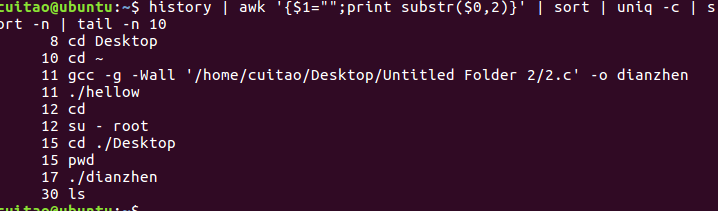
\includegraphics[width=0.5\linewidth]{常用的十条指令.png}
    \caption{常用的十条指令}
    \label{fig:enter-label}
\end{figure}

3.终端多路复用tmux会话操作。

   
\begin{itemize}
    \item \verb|tmux| 开始一个新的会话
    \item \verb|tmux new -s NAME| 以指定名称开始一个新的会话
    \item \verb|tmux ls| 列出当前所有会话
    \item 在 \verb|tmux| 中输入 \verb|<C-b> d| ,将当前会话分离
    \item \verb|tmux a| 重新连接最后一个会话。您也可以通过 \verb|-t| 来指定具体的会话
\end{itemize}
   
4.终端多路复用tmux会话操作

\begin{itemize}
    \item \verb|<C-b> c| 创建一个新的窗口,使用 \verb|<C-d>| 关闭
    \item \verb|<C-b> N| 跳转到第 \textit{N} 个窗口,注意每个窗口都是有编号的
    \item \verb|<C-b> p| 切换到前一个窗口
    \item \verb|<C-b> n| 切换到下一个窗口
    \item \verb|<C-b> ,| 重命名当前窗口
    \item \verb|<C-b> w| 列出当前所有窗口
\end{itemize}
 

5.终端多路复用tmux面板操作

\begin{itemize}
    \item \verb|<C-b> "| 水平分割
    \item \verb|<C-b> %| 垂直分割
    \item \verb|<C-b> <方向>| 切换到指定方向的面板,<方向> 指的是键盘上的方向键
    \item \verb|<C-b> z| 切换当前面板的缩放
    \item \verb|<C-b> [| 开始往回卷动屏幕。您可以按下空格键来开始选择,回车键复制选中的部分
    \item \verb|<C-b> <空格>| 在不同的面板排布间切换
\end{itemize}
 
6.别名的设置
  别名设置的格式为:alias alias\_name="command\_to\_alias arg1 arg2"实际应用例如将ll设置为ls -lh,这样可以简化指令,便于记忆。alias ll="ls -lh"\newline
\begin{figure}
    \centering
    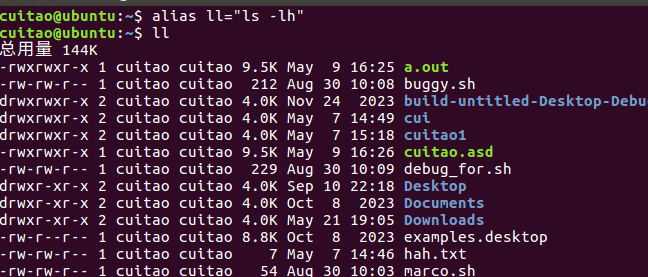
\includegraphics[width=0.5\linewidth]{别名.png}
    \caption{Enter Caption}
    \label{fig:设置别名}
\end{figure}
7.远程设备的连接
\begin{itemize}
    \item 前往 \verb|~/.ssh/| 并查看是否已经存在 SSH 密钥对。如果不存在,请使用 \verb|ssh-keygen -o -a 100 -t ed25519| 来创建一个 
    \item 在 \verb|.ssh/config| 加入下面内容\newline
 Host vm\newline
    User username\_goes\_here\newline
    HostName ip\_goes\_here\newline
    IdentityFile ~/.ssh/id\_ed25519\newline
    LocalForward 9999 localhost:8888\newline
    \item 使用 \verb|ssh-copy-id vm| 将您的 ssh 密钥拷贝到服务器
    \item  使用 \verb|python -m http.server 8888| 在您的虚拟机中启动一个 Web 服务器并通过本机的 \verb|http://localhost:9999| 访问虚拟机上的 Web 服务器
    \item 使用 \verb|sudo vim /etc/ssh/sshd_config| 编辑 SSH 服务器配置,通过修改 \verb|PasswordAuthentication| 的值来禁用密码验证。通过修改 \verb|PermitRootLogin| 的值来禁用 root 登录。然后使用 \verb|sudo service sshd restart| 重启 \verb|ssh| 服务器,然后重新尝试即可连接到虚拟机。
 
\end{itemize}
\newline
8.tmux常用指令
\begin{itemize}
\item tmux ls 会显示出所有正在运行的对话
\item tmux attach -t 0 连接到特定的对话。
\item tmux rename-session -t 0 database 重命名当前会话。
\end{itemize}

9.常见目录说明

\begin{itemize}
    \item /bin:存放\textbf{二进制可执行文件}(ls、cat、mkdir 等),\textbf{常用命令一般都在这里};
    \item /sbin: 存放二进制可执行文件,只有 root 才能访问。这里存放的是系统管理员使用的系统级别的管理命令和程序。如 \verb|ifconfig| 等;
    \item /etc:存放\textbf{系统管理和配置文件};
    \item /root:超级用户(系统管理员)的主目录;
    \item /home:存放所有用户文件的根目录,是用户主目录的基点,比如用户 user 的主目录就是 /home/user,可以用 \~user 表示;
    \item /dev:用于存放\textbf{设备文件};
    \item /usr:用于存放\textbf{系统应用程序};
    \item /lib 和/lib64:存放着\textbf{和系统运行相关的库文件};
\end{itemize}
 



10.
top指令可以查看系统进程和资源占用情况。
\begin{figure}
    \centering
    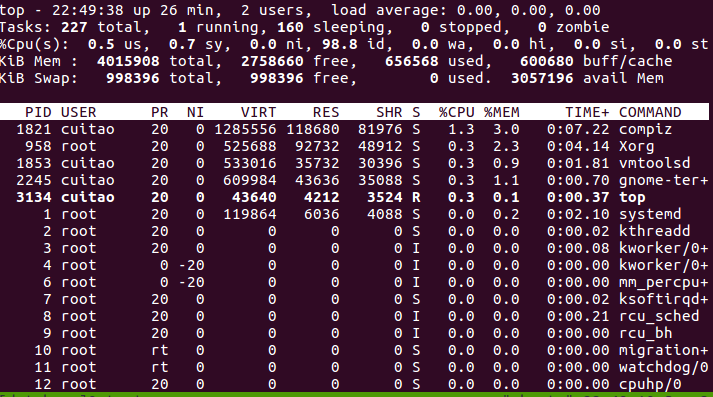
\includegraphics[width=0.5\linewidth]{top.png}
    \caption{top指令查看系统情况}
    \label{fig:enter-label}
\end{figure}



\subsection{Python学习例子10个}
1.python实现字符串编码解码操作。
    编码是将字符串转换为二进制数据bytes
    ;而解码则是将bytes类型的数据转换成字符串类型

\noindent
\begin{minipage}{\linewidth}
  \centering
  % 插入图片
  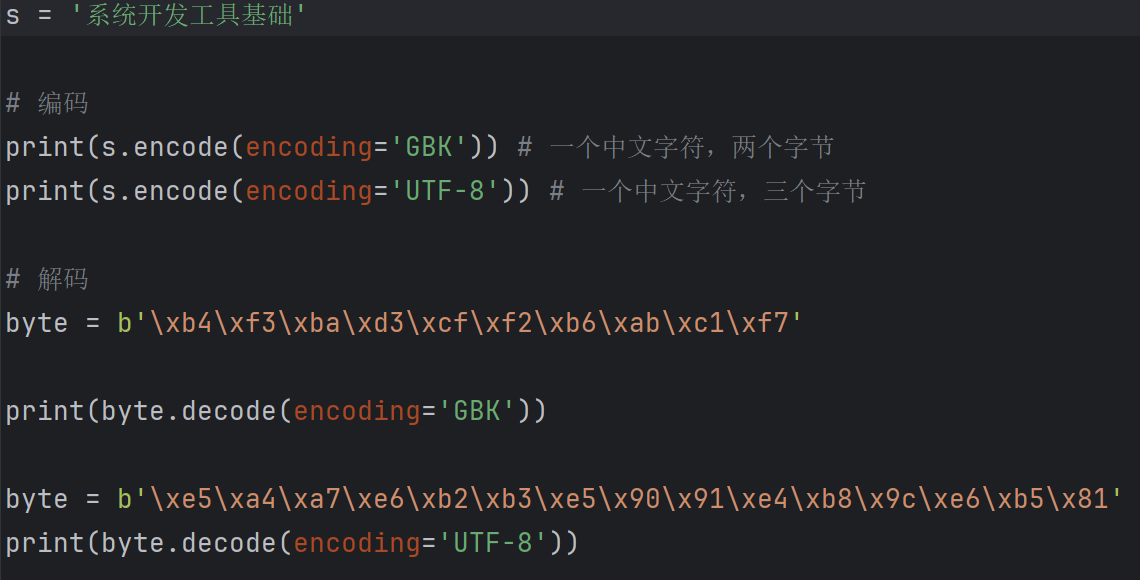
\includegraphics[width=0.5\linewidth]{Python编码解码.png}
  % 图片标题
  \captionof{figure}{Python编码解码}
  \label{fig:example}
\end{minipage}


2.Python实现文件读写\newline
\noindent
\begin{minipage}{\linewidth}
  \centering
  % 插入图片
  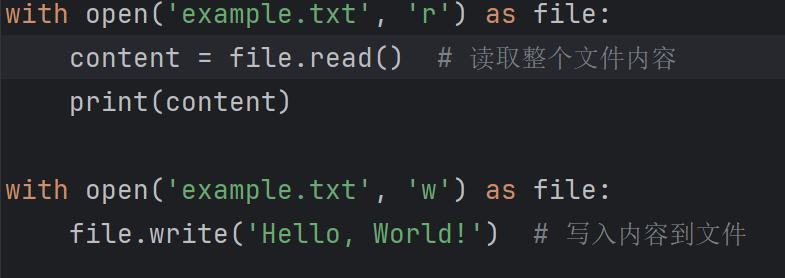
\includegraphics[width=0.5\linewidth]{Python文件读写.png}
  % 图片标题
  \captionof{figure}{文件读写}
  \label{fig:example}
\end{minipage}

3.Python实现自定义函数,从而实现有效的代码复用。

\noindent
\begin{minipage}{\linewidth}
  \centering
  % 插入图片
  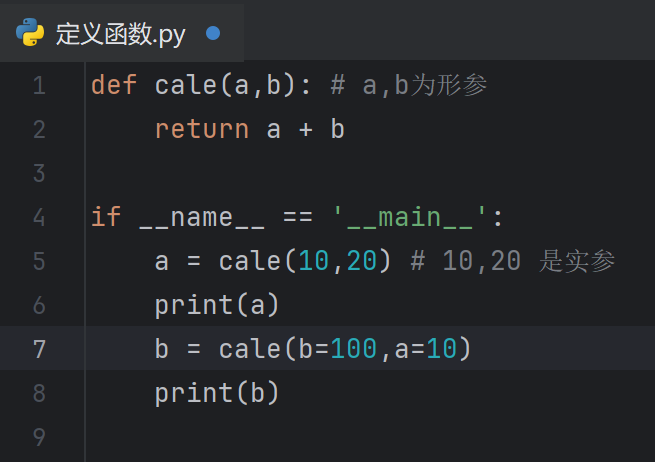
\includegraphics[width=0.5\linewidth]{自定义函数.png}
  % 图片标题
  \captionof{figure}{Python函数的定义}
  \label{fig:example}
\end{minipage}

4.Python常见抛出的异常类型

\begin{itemize}
\item ZeroDivisionError \#除或取模零的类型
\item  IndexError \#序列中没有此索引 
\item KeyError \#映射中没有这个键 
\item NameError \#未声明/初始化对象(没有属性) 
\item SyntaxError \#Python语法错误 
\item ValueError \#传入无效的参数 
\end{itemize}
\newline 使用try和except来抛出和捕获异常,保证程序正确运行。\newline
\noindent
\begin{minipage}{\linewidth}
 \centering
  % 插入图片
  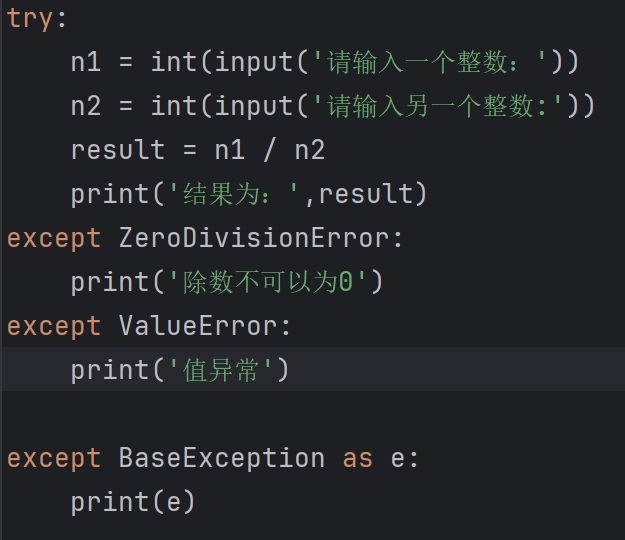
\includegraphics[width=0.5\linewidth]{异常处理.png}
  % 图片标题
  \captionof{figure}{Python异常处理}
  \label{fig:example}
\end{minipage}

5.
Python类的声明定义

\begin{figure}
    \centering
    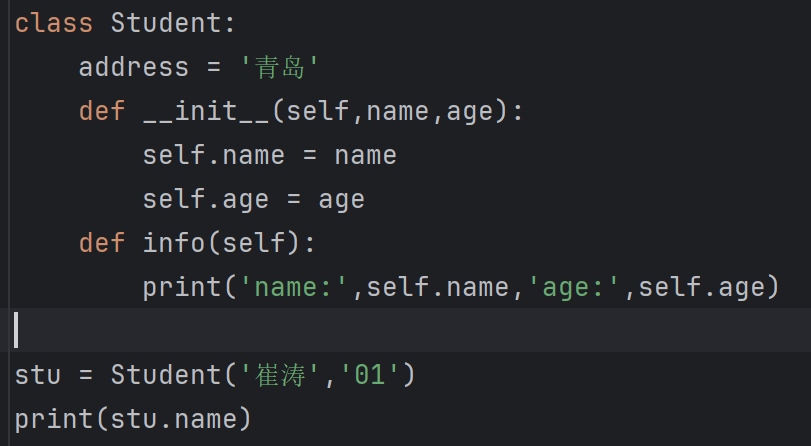
\includegraphics[width=0.5\linewidth]{类的声明定义.png}
    \caption{类的声明定义}
    \label{fig:enter-label}
\end{figure}

6.通过pip install 模块名 ,可以安装第三方模块,避免重复造轮子。\newline
7.切换颜色向输出台打印文字:print('\textbackslash{}033[0:35m\textbackslash{}t\textbackslash{}tPython切换颜色打印\textbackslash{}033[m') 
\newline
8.python通过循环来实现冒泡排序

\noindent
\begin{minipage}{\linewidth}
 \centering
  % 插入图片
  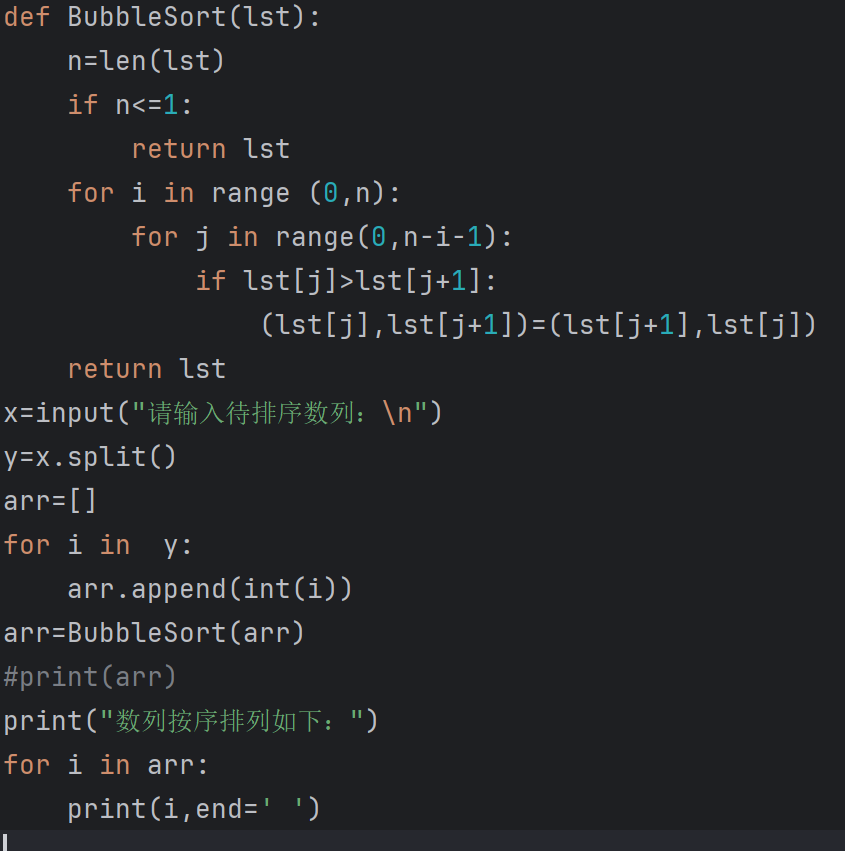
\includegraphics[width=0.5\linewidth]{冒泡排序.png}
  % 图片标题
  \captionof{figure}{冒泡排序}
  \label{fig:example}
\end{minipage}

9. 字典数据结构\newline
字典的一般形式为d = \{key1 : value1, key2 : value2 \} \newline
值可以取任何数据类型,但键必须是不可变的,如字符串,数字或元组。 
\newline
10.求解斐波那契数列第n项

\noindent
\begin{minipage}{\linewidth}
 \centering
  % 插入图片
  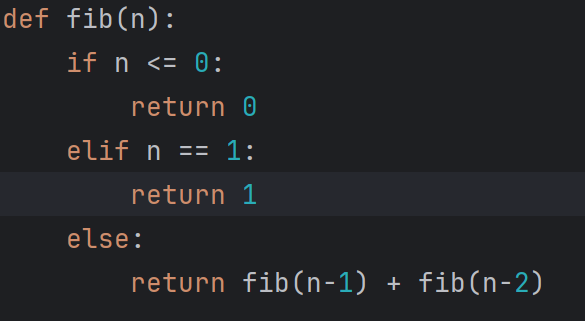
\includegraphics[width=0.5\linewidth]{斐波那契.png}
  % 图片标题
  \captionof{figure}{求解斐波那契数列}
  \label{fig:example}
\end{minipage}




\section{收获感悟}
通过学习命令行环境,我学会了编写简单的脚本,来实现一些基本的文件管理、数据处理等,极大地提高了日常效率。同时我还学会了如何远程连接虚拟机,这样方便远程协作。通过学习tmux,我学会了多视窗协作,大大方便了以后的工作。
学习Python最喜欢的就是它的库。我发现无论是爬虫还是机器学习,Python都有相应的第三方库来简化,大大降低了难度,更加容易上手,但是我又发现Python程序的运行时间普遍是要长于之前学习过的c语言,我想这应该是Python的一个缺陷。
通过Python和命令行环境这俩的综合学习,我明白了如何通过命令行运行Python脚本,如何利用Python来处理命令行中的文本和数据,大大提高了效率。

github路径
您可以在此查看项目的源代码: 

\url{https://github.com/cuitao223/homework3}
\end{document}
